
\section{Second approach to the FSM}

\subsection{Staggered meshes}

In order to solve the decoupling of the velocity and pressure fields, two strategies have been developed, namely staggered meshes and collocated meshes. Nonetheless, we shall focus only on the former, more specifically, in the case of cartesian meshes. 

In a staggered mesh, rather than locating the pressure and velocity terms at the same point in space as we have done so far, these pressure is set at the centre of the control volume whereas the velocity components are located at the faces of the control volume, as Figure \ref{fig:staggered_mesh} shows.

\begin{figure}[h]
    \centering
    \begin{tikzpicture}
        \def\lx{3cm}
        \def\ly{1.85cm}
        \def\velocitylength{1cm}

        % Grid
        \draw[] (0,0) rectangle (3*\lx,3*\ly);
        \draw[] (1*\lx,0) -- ++(0,3*\ly);
        \draw[] (2*\lx,0) -- ++(0,3*\ly);
        \draw[] (0,1*\ly) -- ++(3*\lx,0);
        \draw[] (0,2*\ly) -- ++(3*\lx,0);

        % Nodes
        \begin{scope}[shift={(0.5*\lx,0.5*\ly)}]
            \foreach \x in {0,1,2} {
                \foreach \y in {0,1,2} {
                    \filldraw[] ({\x*\lx},{\y*\ly}) circle (2pt);
                }
            }
        \end{scope}

        

        % No stagg CV
        \begin{scope}[shift={(\lx,\ly)}]
            \fill[blackcv] (0,0) rectangle ++(\lx,\ly);
            \draw[blackfill] (0,0) rectangle ++(\lx,\ly);
            % Node P
            \node[anchor=north east] at ({0.5*\lx}, {0.5*\ly}) {$P$};
        \end{scope}


        % Stagg-x CV
        \begin{scope}[shift={(1.5*\lx,\ly)}]
            % Control volume
            \fill[bluecv] (0,0) rectangle ++(\lx,\ly);
            \draw[bluefill] (0,0) rectangle ++(\lx,\ly);
            % Velocity
            \node[anchor=south, blue] at ({0.5*\lx+0.5*\velocitylength},{0.5*\ly}) {$u$};
        \end{scope}

        % Stagg-y CV
        \begin{scope}[shift={(\lx,1.5*\ly)}]
            % Control volume
            \fill[redcv] (0,0) rectangle ++(\lx,\ly);
            \draw[redfill] (0,0) rectangle ++(\lx,\ly);
            % Velocity
            \node[anchor=west, red] at ({0.5*\lx},{0.5*\ly+0.5*\velocitylength}) {$v$};
        \end{scope}

        % Velocity u
        \begin{scope}[shift={(0,0.5*\ly)}]
            \foreach \x in {0,...,3} {
                \foreach \y in {0,1,2} {
                    \draw[velocity] ({\x*\lx-0.5*\velocitylength},\y*\ly) -- ++(\velocitylength,0);
                }
            }
        \end{scope}

        
        % Velocity v
        \begin{scope}[shift={(0.5*\lx,0)}]
            \foreach \x in {0,1,2} {
                \foreach \y in {0,...,3} {
                    \draw[velocity, red] (\x*\lx,{\y*\ly-0.5*\velocitylength}) -- ++(0,\velocitylength);
                }
            }
        \end{scope}


    \end{tikzpicture}
    \caption{Staggered mesh. Source: adapted from \colorbox{red}{asdas}}
    \label{fig:staggered_mesh}
\end{figure}


\begin{figure}[h]
    \centering
    
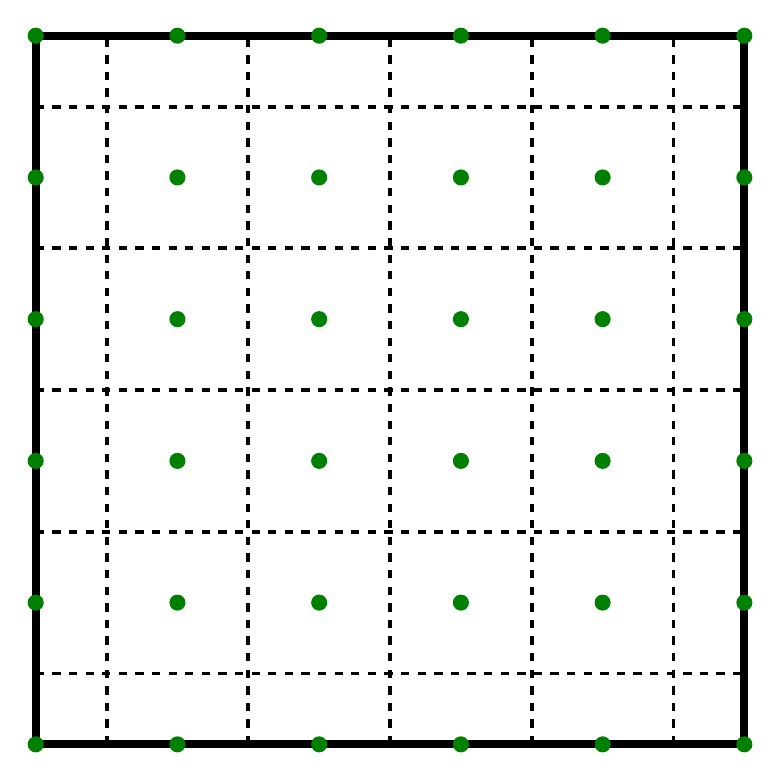
\begin{tikzpicture}[scale=0.9]
    \def\Lx{10cm}
    \def\Ly{10cm}
    \def\velocitylength{1.5cm}
    \draw[line width=1mm] (0,0) rectangle (\Lx,\Ly);

    % Nodes
    \foreach \x in {0,...,5} {
        \foreach \y in {0,...,5} {
            \filldraw[green!50!black] (2*\x,2*\y) circle (3pt);
        }
    }

    \begin{scope}[shift={(1,0)}]
        \foreach \x in {0,...,4} {
            \draw[line width=0.5mm, dashed] (2*\x,0) -- ++(0,\Ly);
        }
    \end{scope}

    % Control volume boundaries y
    \begin{scope}[shift={(0,1)}]
        \foreach \y in {0,...,4} {
            \draw[line width=0.5mm, dashed] (0,2*\y) -- ++(\Lx,0);
        }
    \end{scope}
\end{tikzpicture}
    \caption*{Pressió: cares centrades.}
    \vspace{0.7cm}
    \begin{tikzpicture}[scale=0.9]
    \def\Lx{10cm}
    \def\Ly{10cm}
    \def\velocitylength{1.5cm}

    \fill[black!50!white, opacity=0.5] (-1,-1) rectangle (\Lx + 1 cm,\Ly + 1 cm);
    \fill[white] (0,0) rectangle (\Lx,\Ly);

    \draw[line width=1mm] (0,0) rectangle (\Lx,\Ly);

    % Nodes
    \foreach \x in {0,...,5} {
        \foreach \y in {0,...,5} {
            \filldraw[green!50!black] (2*\x,2*\y) circle (3pt);
        }
    }

    % Control volumes boundaries
    \begin{scope}[shift={(-1,-1)}]
        \foreach \x in {0,...,6} {
            \draw[line width=0.5mm, dashed] (2*\x,0) -- ++(0,\Ly+2cm);
        }
        \foreach \y in {0,...,6} {
            \draw[line width=0.5mm, dashed] (0,2*\y) -- ++(\Lx+2cm,0);
        }
    \end{scope}

    % Velocity u
    \begin{scope}[shift={(1,0)}]
        \foreach \x in {-1,...,5} {
            \foreach \y in {0,...,5} {
                \draw[velocity, line width=0.5mm] ({2*\x cm - 0.5*\velocitylength},2*\y) -- ++(\velocitylength,0);
            }
        }
    \end{scope}

    % Velocity v
    \begin{scope}[shift={(0,-1)}]
        \foreach \x in {0,...,5} {
            \foreach \y in {0,...,6} {
                \draw[velocity, line width=0.5mm, red] (2*\x,2*\y cm - 0.5*\velocitylength) -- ++(0,\velocitylength);
            }
        }            
    \end{scope}
\end{tikzpicture}
    \caption*{Pressió: cares centrades. Velocitat $u$: staggered--$x$. Velocitat $v$: staggered--$y$.}
\end{figure}


\clearpage
\begin{figure}[h]
    \centering
    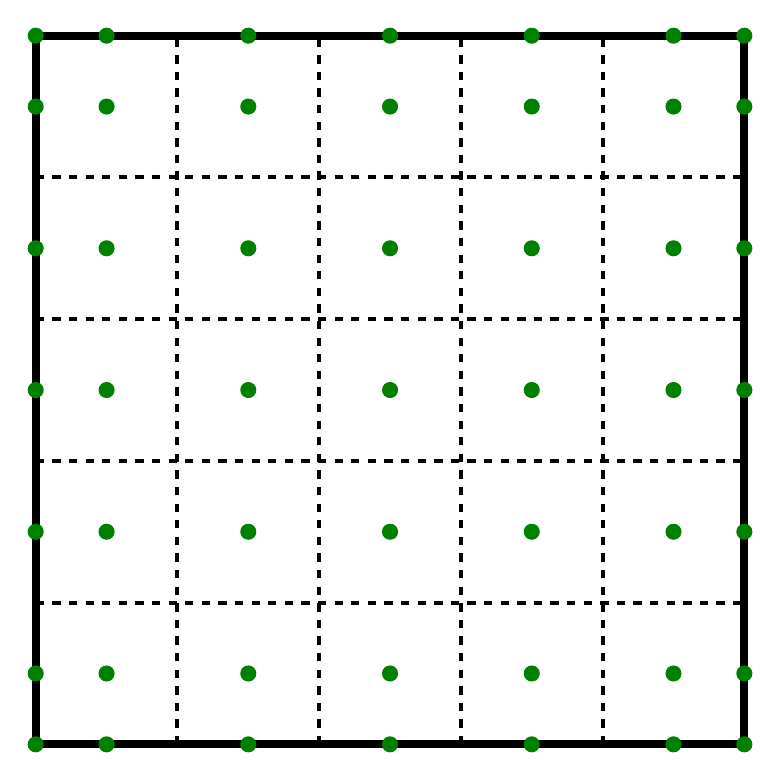
\begin{tikzpicture}[scale=0.9]
    \def\Lx{10cm}
    \def\Ly{10cm}
    \def\velocitylength{1.5cm}
    \draw[line width=1mm] (0,0) rectangle (\Lx,\Ly);

    % Control volume boundaries
    \foreach \x in {1,...,4} {
        \draw[line width=0.5mm, dashed] (2*\x,0) -- ++(0,\Ly);
    }

    \foreach \y in {1,...,4} {
        \draw[line width=0.5mm, dashed] (0,2*\y) -- ++(\Lx,0);
    }

    % Nodes
    \begin{scope}[shift={(1,0)}]
        \foreach \x in {0,...,4} {
            \foreach \y in {0,...,4} {
                \filldraw[green!50!black] (2*\x,2*\y cm + 1 cm) circle (3pt);
            }
        }
    \end{scope}

    % Boundary nodes
    \foreach \y in {0,1} {
        \filldraw[green!50!black] (0,\y*\Ly) circle (3pt);
        \filldraw[green!50!black] (\Lx,\y*\Ly) circle (3pt);
        \begin{scope}[shift={(1,0)}]
            \foreach \x in {0,...,4} {
                \filldraw[green!50!black] (2*\x,\y*\Ly) circle (3pt);
            }
        \end{scope}
    }
    \begin{scope}[shift={(0,1)}]
        \foreach \x in {0,1} {
            \foreach \y in {0,...,4} {
                \filldraw[green!50!black] (\x*\Lx,2*\y cm) circle (3pt);
            }
        }
    \end{scope}

\end{tikzpicture}
    \caption*{Pressió: nodes centrats.}
    \vspace{0.7cm}
    \begin{tikzpicture}[scale=0.9]
    \def\Lx{10cm}
    \def\Ly{10cm}
    \def\velocitylength{1.5cm}
    \draw[line width=1mm] (0,0) rectangle (\Lx,\Ly);

    % Control volume boundaries
    \foreach \x in {1,...,4} {
        \draw[line width=0.5mm, dashed] (2*\x,0) -- ++(0,\Ly);
    }

    \foreach \y in {1,...,4} {
        \draw[line width=0.5mm, dashed] (0,2*\y) -- ++(\Lx,0);
    }

    % Nodes
    \begin{scope}[shift={(1,0)}]
        \foreach \x in {0,...,4} {
            \foreach \y in {0,...,4} {
                \filldraw[green!50!black] (2*\x,2*\y cm + 1 cm) circle (3pt);
            }
        }
    \end{scope}

    % Boundary nodes
    \foreach \y in {0,1} {
        \filldraw[green!50!black] (0,\y*\Ly) circle (3pt);
        \filldraw[green!50!black] (\Lx,\y*\Ly) circle (3pt);
        \begin{scope}[shift={(1,0)}]
            \foreach \x in {0,...,4} {
                \filldraw[green!50!black] (2*\x,\y*\Ly) circle (3pt);
            }
        \end{scope}
    }
    \begin{scope}[shift={(0,1)}]
        \foreach \x in {0,1} {
            \foreach \y in {0,...,4} {
                \filldraw[green!50!black] (\x*\Lx,2*\y cm) circle (3pt);
            }
        }
    \end{scope}

    % Velocity u
    \foreach \y in {0,1} {
        \foreach \x in {0,...,5} {
            \draw[velocity, line width=0.5mm] (2*\x cm -0.5*\velocitylength,\y*\Ly) -- ++(\velocitylength,0);
        }
    }
    \begin{scope}[shift={(0,1)}]
        \foreach \y in {0,...,4} {
            \foreach \x in {0,...,5} {
                \draw[velocity, line width=0.5mm] (2*\x cm -0.5*\velocitylength,2*\y) -- ++(\velocitylength,0);
                
            }
        }
    \end{scope}

    % Velocity v
    \foreach \x in {0,1} {
        \foreach \y in {0,...,5} {
            \draw[velocity, line width=0.5mm, red] (\x*\Lx,2*\y cm - 0.5*\velocitylength) -- ++(0,\velocitylength);
        }
    }
    \begin{scope}[shift={(1,0)}]
        \foreach \x in {0,...,4} {
            \foreach \y in {0,...,5} {
                \draw[velocity, line width=0.5mm, red] (2*\x,2*\y cm - 0.5*\velocitylength) -- ++(0,\velocitylength);
            }
        }
    \end{scope}

\end{tikzpicture}
    \caption*{Pressió: nodes centrades. Velocitat $u$: staggered--$x$. Velocitat $v$: staggered--$y$.}
\end{figure}

